\chapter{肝移植围手术期管理}

\section{前沿学术综述}

自1963年在人体成功地完成了世界第一例肝脏移植到现在,全球接受肝移植患者已达6万例,最长生存达29年。我国肝移植事业虽然起步较晚,但发展较快。1977年我国仅有2家单位共完成2例肝移植手术(不包括港澳台地区),而到2005年底,据中华器官移植杂志和全国肝移植协作组统计,我国肝移植累计完成例数已经超过8000例,仅2005年一年就施行了约3000例。肝移植作为目前治疗终末期肝病的唯一有效手段已被社会各界所接受。在经历了两次发展高潮以后,我国肝移植正逐步进入平稳发展期,这一阶段不再是单纯追求例数的增加,而是从提高术后长期存活率等多个层次提出更高的要求。

术前(Child-Turcotte-Pugh,Child评分)和(Unite Network for Organ
Sharing,美国纽约器官分级)分级曾经被广泛地用于供肝的合理分配,但该类分级所包含的等级较少,同一等级内可能会有大量患者,所以有时较难决定谁更需优先手术。2002年2月美国纽约器官分级将终末期肝病模型(Model
for End-stage Liver Disease)作为成人肝移植的新标准。Onaca等
\protect\hyperlink{text00020.htmlux5cux23ch1-19}{\textsuperscript{{[}1{]}}}
根据移植前的评分将患者分为<15、15~24、>25分3个层面,发现术后3、6、12、18及24个月生存率与终末期肝病模型评分有明显关系,分值越高患者移植后生存率越低。美国梅奥医学中心(Mayo
Medical Center)的Patrick认为
\protect\hyperlink{text00020.htmlux5cux23ch2-19}{\textsuperscript{{[}2{]}}}
,终末期肝病模型评分>24或终末期肝病模型评分>18伴有全身炎症反应综合征是慢性肝脏疾病急性加重致肝衰竭患者肝移植后死亡的高风险因素。因此移植前行终末期肝病模型评分对预测肝移植术后患者生存率有一定的意义。

Douglas等
\protect\hyperlink{text00020.htmlux5cux23ch3-19}{\textsuperscript{{[}3{]}}}
指出,终末期肝病模型评分<21时,终末期肝病模型评分、低钠血症和持续性的腹水均是患者早期死亡率的预测因子,当终末期肝病模型评分>21分时,仅仅终末期肝病模型分级本身是患者预后预测因子。众多研究
\protect\hyperlink{text00020.htmlux5cux23ch4-19}{\textsuperscript{{[}4{]}}}
\textsuperscript{~}
\protect\hyperlink{text00020.htmlux5cux23ch6-19}{\textsuperscript{{[}6{]}}}
表明,水和钠潴留是终末期肝病严重程度的决定因子和预后预测因子。血清钠值是对于终末期肝病患者待肝期间预后的良好预测指标。最近有学者指出,在部分伴有持续腹水、低钠血症(血清钠<135mmol/L)的患者中,虽然终末期肝病模型评分较低,却有较高的移植前死亡率。并且随着低钠血症的进一步恶化,死亡危险度逐渐增加
\protect\hyperlink{text00020.htmlux5cux23ch3-19}{\textsuperscript{{[}3{]}}}
。因此提出了终末期肝病模型---Na的概念。将血清钠应用于对终末期肝病患者预后评估的研究较多,其中来自我国台湾省的Teh-laHuo等
\protect\hyperlink{text00020.htmlux5cux23ch7-19}{\textsuperscript{{[}7{]}}}
提出了“终末期肝病模型评分/血清钠比率指数”,即“MESO指数”将终末期肝病模型评分/血清钠值用于评估肝硬化患者的预后。作者认为,终末期肝病模型评分/血清钠比率指数,可以预测肝硬化患者的近期和远期预后。但是,终末期肝病模型评分/血清钠比率指数本身具有分布范围狭窄的特点,故其在实际应用过程中具有一定的局限性。

随着肝移植例数的逐年增加,供体不足的问题已成为制约肝移植发展的瓶颈之一。肝移植手术的适应证逐步扩大,肝源则日益紧张,移植学家们为肝源的有效利用及新肝源的开拓也尝试了多种新移植术式,扩展供肝来源的方式也越来越多。这其中包括通过外科技术的进步而开展活体肝移植及劈离式肝移植、通过中国捐献体系的建立从而使供肝捐献数量增多、以及扩大标准供肝即边缘供肝的使用。

1989年Strong等
\protect\hyperlink{text00020.htmlux5cux23ch8-19}{\textsuperscript{{[}8{]}}}
利用成人左外侧叶肝对一个胆道闭锁的患儿成功实施了世界首例活体肝移植,1994年Yamaoka等
\protect\hyperlink{text00020.htmlux5cux23ch9-19}{\textsuperscript{{[}9{]}}}
成功开展了首例成人活体右半肝移植。进入21世纪,活体部分肝移植在全球范围内得到迅猛发展。依据中国肝移植注册系统统计数据,2007和2008年活体移植例数达到峰值,每年均达到400例以上,各占全年移植例数的19%或以上。截止2010年6月,国内共完成1483例活体肝移植,活体肝移植技术也随之日趋成熟。虽然活体肝移植能够取得良好的效果,但仍需重视活体肝移植受者的并发症。研究表明,胆道并发症是活体肝移植最常见的并发症,发生率为15%~30%,其中胆漏是最常见的并发症。肝动脉栓塞以及腹腔感染的发生率均高于尸体肝移植,而熟练的技术能够在很大程度上减少并发症的发生
\protect\hyperlink{text00020.htmlux5cux23ch10-19}{\textsuperscript{{[}10{]}}}
。

自体肝移植已有20余年历史,但开展很少。德国Pichlmayer教授于1988年最早实施自体肝移植
\protect\hyperlink{text00020.htmlux5cux23ch11-19}{\textsuperscript{{[}11{]}}}
,随后Hannoun等对该技术进行了改进和简化。自体移植是目前肝脏外科难度系数最高、最需多学科共同协作的一种外科技术,中国2005~2007年间仅开展8例。

多米诺肝移植是一种针对家族性淀粉样多发性神经病(familial amyloidotic
polyneuropathy,FAP)的手术术式。原位肝移植1990年被用于治疗FAP,并成为目前治疗该病的唯一方法。来自西班牙1999/2009肝移植统计网的数据显示,多米诺肝移植后的生存率稍高于尸体肝移植和活体肝移植。中国自2006年开展第1例多米诺肝移植,目前开展很少。

劈离式肝移植最早由Pichelmayr和Bismuth提出,并逐渐在世界各大移植中心开展。劈离式肝移植最常应用于一个成人受者和儿童,目前也越来越多应用于成人之间。随着劈离式肝移植技术的进步和手术医生水平的提高,采用劈离式肝移植的术后生存率不断提高,术后发生血管和胆道并发症的风险也在可接受的范围内
\protect\hyperlink{text00020.htmlux5cux23ch12-19}{\textsuperscript{{[}12{]}}}
。Yersiz等
\protect\hyperlink{text00020.htmlux5cux23ch13-19}{\textsuperscript{{[}13{]}}}
研究发现,该机构1991/2005间进行的110例劈离式肝移植,受体存活率、移植物存活率与全肝移植相当。来自英国的King'sCollegeHospital在1994~2000年为80例儿童实施劈离式肝移植。随访研究表明:术后1、3年受者生存率分别为93.5%和88.1%,移植物存活率为89.7%和86.1%。而肝血管并发症及胆道并发症发生率分别仅为7.5%和8.7%,与全肝移植相当
\protect\hyperlink{text00020.htmlux5cux23ch14-19}{\textsuperscript{{[}14{]}}}
。目前,劈离式肝移植在欧洲和澳洲开展较多,并逐渐扩展到双成人受者的肝移植,开展处于上升趋势。而国内2002年开展第一例劈离式肝移植,截止到2009年,仅进行72例
\protect\hyperlink{text00020.htmlux5cux23ch15-19}{\textsuperscript{{[}15{]}}}
。

辅助性肝移植能帮助急性肝衰竭的患者稳妥地渡过肝衰竭期,待受体原肝(native
liver,NL)肝细胞再生和肝功能恢复正常后可停用免疫抑制剂。辅助性肝移植的常用术式主要有3类,其中,辅助性部分原位肝移植(auxiliary
partial orthotopic liver
transplantation)现在已经成为肝移植的标准术式。该方法将原左半肝或右半肝切除,再植入劈裂的部分供肝于原位。随着手术方式的改进和上述各种技术问题的解决,辅助性肝移植的适应证将不断扩大,与原位肝移植互为补充。

心死亡供体近几年也开始有所增加。心脏死亡器官捐献(donation after cardiac
death)始于美国。1995年Pittsburgh和Madison的医疗团队首先报道了心脏死亡器官捐献移植案例
\protect\hyperlink{text00020.htmlux5cux23ch16-19}{\textsuperscript{{[}16{]}}}
\textsuperscript{,}
\protect\hyperlink{text00020.htmlux5cux23ch17-19}{\textsuperscript{{[}17{]}}}
。2009年11月底,中国红十字会总会在北京召开了心脏死亡器官捐献试点工作研讨会,会上决定制定心脏死亡器官捐献工作指南。随后,全国人体器官捐献试点工作正式开展。天津、浙江、广东等11个省市成为首批试点地区。截至2012年2月29日,通过人体器官捐献试点工作渠道,我国大陆实现心脏死亡器官捐献共196例,捐献大器官511个(其中肝脏161个、肾脏342个、心脏5个、肺3个)。

国外资料显示,应用心脏死亡器官捐献供体能够增加8%的移植数量,甚至能够达到25%
\protect\hyperlink{text00020.htmlux5cux23ch18-19}{\textsuperscript{{[}18{]}}}
。既往文献报道心脏死亡器官捐献供体原发性移植物失功的发生率高达12%,胆道并发症的发生率高达60%
\protect\hyperlink{text00020.htmlux5cux23ch19-19}{\textsuperscript{{[}19{]}}}
。而近来报道显示心脏死亡器官捐献供体并发症的发生率并不高于其他类别的供体。通过可控的程序性撤除生命支持所获得的心脏死亡器官捐献供体,其1年的患者和移植物存活率可高达100%,3年存活率分别为89.5%和68.4%,5年存活率分别为89.5%和63.2%
\protect\hyperlink{text00020.htmlux5cux23ch20-19}{\textsuperscript{{[}20{]}}}
。

在原位肝移植术后开始阶段,较典型的血流动力学状态是高心排出量、低体循环阻力及高氧输送状态,少有完全正常的血流动力学状态。如果患者早期不出现高血流动力学状态,常常病死率较高。血容量过多、右房压过高易导致肝淤血,对供肝造成损害。在2011年6月于西班牙举行的第17届国际肝移植学会(International
Liver Transplantation
Society)上,有专家认为在移植部分供肝时监测受者血流动力学是很有必要的
\protect\hyperlink{text00020.htmlux5cux23ch2-19}{\textsuperscript{{[}2{]}}}
。为避免开通血流即刻出现过高的灌注压,在处理时需考虑受者原始肝脏的门静脉压、临时性门腔静脉分流时的门静脉血流数据,有效的入肝血流调节有利于减小部分移植肝的体积。

关于移植术后感染方面,参加此次会议的法国巴黎第11大学(Université Paris
Ⅺ)Faouzi
Saliba教授则指出,感染是肝移植后受者死亡的主要原因,其中革兰阳性菌感染占69.1%,侵袭性真菌感染也不少见。巨细胞病毒感染使移植后1年受者病死率增加。一些移植中心还出现了较多的耐药菌株,如抗甲氧西林金黄色葡萄球菌、抗万古霉素肠球菌。出现耐药菌的风险因素包括抗生素使用史、反复住院、有创操作、二次移植和胆道并发症等。加强控制感染的措施包括对受者和环境进行微生物监测、对机会性感染进行预防和给予抢先治疗等。

另外一个常见并发症是代谢综合征。近年发生率呈逐渐上升的趋势,其中丙型病毒性肝炎和非酒精性脂肪肝病是重要的危险因素。移植后代谢综合征与移植后心血管疾病、终末期肾病、进展性丙型病毒性肝炎和恶性肿瘤的发生相关。防治措施包括监测血脂、血压和控制慢性肾病,以及进行减肥手术。

在免疫抑制剂的进展方面。免疫抑制剂的使用更加规范化,关于移植后免疫耐受的研究一直都是移植学专家们热衷的领域。一项关于可控性耐受在儿童和成人肝移植中的诊断和预测价值的研究发现,至少13个外周血中的基因组能预测成人和儿童可控性耐受的表型,其中在儿童中的预测更好。

此外,对术后如何预防乙型肝炎和丙型肝炎的复发以及肿瘤的复发也一直受到关注。乙型肝炎免疫球蛋白联合核苷类抗病毒药物,可以使移植术后乙型肝炎的复发和乙型肝炎变异问题得到部分解决,但对丙型肝炎的复发和移植肝内肝外肿瘤复发尚未找到满意的解决方法,也是尚待解决的难题。

另外,影像学在肝移植围手术期发挥越来越重要的作用,尤其是准确的供体影像学评估是开展活体肝移植的先决条件,也应进一步强化其在围手术期处理中的地位。

总之,随着新的移植术式的不断发展,以及供肝肝源多途径的扩展,肝移植患者的围手术期管理显得更为重要。更应该从供肝的获取、保存、植入以及术后管理等各个环节采取有效的措施,最大程度减少各种并发症的发生。

\section{临床问题}

\subsection{肝脏移植围手术期器官功能障碍}

\subsubsection{如何判断移植肝的活力?什么是原发性移植肝无功能?如何诊断?}

移植手术完成后,植入新肝功能能否恢复及恢复时间是人们最为关心的问题。通常情况下,肝功能在72~96小时内迅速改善至正常或接近正常水平
\protect\hyperlink{text00020.htmlux5cux23ch21-19}{\textsuperscript{{[}21{]}}}
。

移植肝无活力的判断有以下几点:①早期出现肝脏功能衰竭表现,钾离子浓度明显增高,代谢性酸中毒,急性低血糖,持续加重的凝血机制障碍,如术中留置T管,则胆汁呈水样或明显减少或消失,但目前由于手术方式的改进,T管已经基本不常规留置;②如为急性排斥,则表现为手术5~7天以后发热、食欲不振、腹部钝痛、精神症状、腹水、肝功能异常、血胆红素升高、凝血机制障碍等,急性排斥反应应通过移植肝活检证实;③多普勒超声检查确认肝血流状态,如有异常应行肝动脉造影、经T管胆管造影、腹部CT等检查确诊。

移植肝无活力的常见原因包括:①原发性移植肝无功能,多系缺血损伤,供肝冷、热缺血时间过长,肝脏感染(细胞或病毒)或药物损害等多因素所致;②技术因素引起术后出血、血管吻合口的栓塞、肝动脉血栓形成或胆道梗阻等;③出现严重的排斥反应。

原发性移植肝无功能(primary liver graft
nonfunction)一般指移植肝脏血流恢复后即可发生的无明确病因导致的移植肝的功能衰竭,需要紧急行再移植术,否则受体死亡则不可避免。其他病因不明的术后早期肝功能不良定义为初期的移植肝功能不良(initial
poor
function)。美国纽约器官分级为了更好的进行移植器官的分配,提出了以下诊断标准(表\ref{tab14-1}),并将发病时间延长到术后10天,可供参考。

\begin{table}[htbp]
\centering
\caption{美国纽约器官分级原发性移植肝无功能诊断标准(成人)}
\label{tab14-1}

\includegraphics{./images/Image00109.jpg}
\end{table}

美国JohnsHopkins提出初期移植肝功能不良的5个诊断标准:①转氨酶升高,提示持续加重的肝损害;②大量补充新鲜冰冻血浆,但国际标准化凝血酶原时间仍持续升高,提示肝脏合成功能恶化;③胆汁分泌量减少且稀薄;④血氨升高,提示肝脏代谢功能无法恢复;⑤彩色超声多普勒发现移植肝血流缓慢。在初期移植肝功能不良的基础上,若术后3天上述情况无改善,则原发性移植肝无功能的发生往往不可避免
\protect\hyperlink{text00020.htmlux5cux23ch22-19}{\textsuperscript{{[}22{]}}}
\textsuperscript{,}
\protect\hyperlink{text00020.htmlux5cux23ch23-19}{\textsuperscript{{[}23{]}}}
。

此外,活体肝移植术后出现的小肝综合征(small-for-sizesyndrome)也被认为是一种特殊类型的原发性移植肝无功能。

\subsubsection{肝移植患者血流动力学有何特点?}

肝移植患者有着自身的特殊性:①大部分患者循环动力学变化特征是高排低阻,同时有门脉高压,使门脉系统毛细血管床的滤过压增加,加上存在一定程度肝功能不全,使得血浆白蛋白的合成减少,血浆胶体渗透压降低;另外,体内醛固酮和抗利尿激素的代谢降低,体液经过再分布,第三间隙液增加,而体内液体总量实际不足
\protect\hyperlink{text00020.htmlux5cux23ch24-19}{\textsuperscript{{[}24{]}}}
;②肝移植术中无肝期、新肝期对循环的干预,血流动力学存在不同的变化;③术中及术后大剂量激素的使用引起水钠潴留,如果输液过量可能会加重机体各脏器的水肿。

Manthous等
\protect\hyperlink{text00020.htmlux5cux23ch25-19}{\textsuperscript{{[}25{]}}}
对术后患者的研究证实,术后3天内实现一天或以上的负平衡,生存率明显高于正平衡组。在肝移植术后肺部并发症方面,有研究认为持久的肺水肿是导致肺炎的高危因素,而且大量输液是发生肺水肿的主要原因,其发生机制与毛细血管渗漏所致毛细血管壁损伤、通透性增加、血浆蛋白漏出是一致的。

一般外科手术后36~72小时毛细血管壁通透性逐渐恢复正常,液体治疗中正平衡转为负平衡。而肝移植患者术后需要使用一段时间的激素,特别在术后几天内,激素用量较大,引起水钠潴留,负平衡出现时间将被推迟,所以术后早期应当限制补液并应用利尿药以利于术后早期液体负平衡的实现。

\subsubsection{肝脏移植术后患者的液体管理具体是如何实施的?}

判断液体复苏的标准以血流动力学稳定为基础,以纠正氧代谢紊乱和防止多器官功能障碍综合征为目的。

表\ref{tab14-2}为肝移植术后患者疾病严重程度分类表。此表中,依据高血流动力学状况、低钠血症、营养不良、门肺高压和心功能不全的存在与否及严重程度将患者分为4类。尽管此分类并未在临床试验中得以检验,但它确实帮助临床医师大致评估肝移植术后患者状况并据此给予重症监护治疗。例如Ⅰ类患者通常对液体治疗的反应近于正常,较Ⅱ类患者需要较少的液体补充。而Ⅱ类患者因慢性肝脏疾病更严重,会通过腹腔引流丢失更多的腹水和蛋白,需要更积极的纠正体液和蛋白损失的相应治疗。Ⅲ类和Ⅳ类患者则产生大量的腹水,并伴有一定程度的肾衰竭,对此类患者纠正其少尿和低血压的治疗,比Ⅰ类和Ⅱ类患者更需谨慎。水和电解质补充需严密监测以防钠盐和水补充过度,防止分别造成中央脑桥脱髓鞘和心肺损害。患者可承受一定程度的低钠血症,以防血管内液体负荷过多,损害本已脆弱的心肺系统
\protect\hyperlink{text00020.htmlux5cux23ch25-19}{\textsuperscript{{[}25{]}}}
\textsuperscript{~}
\protect\hyperlink{text00020.htmlux5cux23ch28-19}{\textsuperscript{{[}28{]}}}
。

\begin{table}[htbp]
\centering
\caption{肝移植术后患者疾病严重程度分类}
\label{tab14-2}
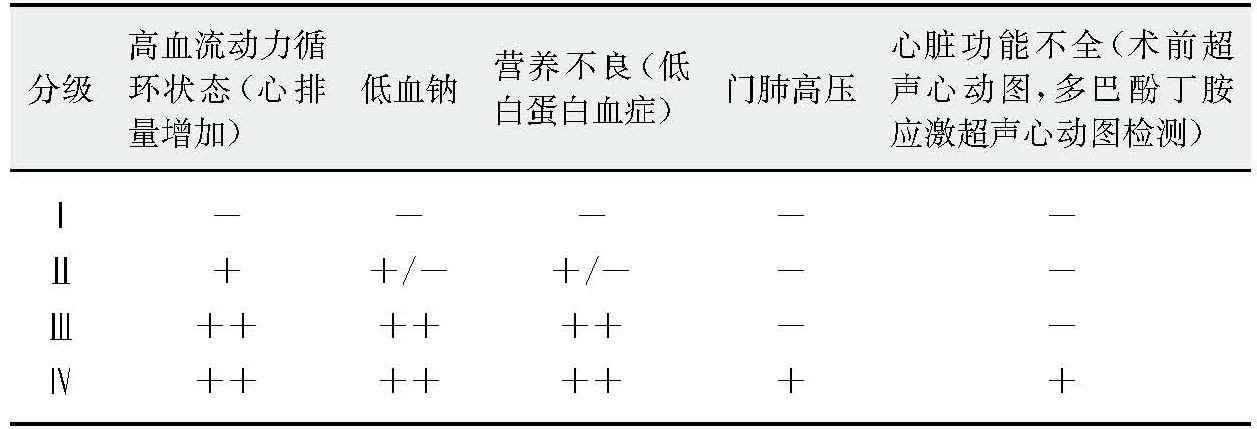
\includegraphics{./images/Image00110.jpg}
\end{table}

肝移植术后早期(24~36小时),由于术中血容量的丢失、大量的第三间隙体液丢失及早期的腹腔引流出大量液体,术后常表现出有效循环血容量明显减少,其监测的方法除了常用的中心静脉压及肺动脉嵌顿压为指标外,还有每搏量变异度(strokevolumevariation)以及被动抬腿试验(passivelegraising,PLR)。每搏量变异度是评估患者血容量状态的敏感指标,也是判断机体对液体治疗反应性的重要指标
\protect\hyperlink{text00020.htmlux5cux23ch29-19}{\textsuperscript{{[}29{]}}}
,可预测循环系统对液体负荷反应性
\protect\hyperlink{text00020.htmlux5cux23ch30-19}{\textsuperscript{{[}30{]}}}
。患者低血容量时每搏量变异度值明显增大,每搏量变异度>10%时提示血容量不足;每搏量变异度<10%时予容量负荷后很难出现心输出量增加,应避免输入过多液体。每搏量变异度、心输出量、心指数、中心静脉压等均用于血容量的判断,其中每搏量变异度与血容量变化的相关性最好
\protect\hyperlink{text00020.htmlux5cux23ch31-19}{\textsuperscript{{[}31{]}}}
。通过对每搏量变异度值分析可预测心血管系统对液体负荷反应的效果,判断其容量状态,对指导血流动力学调控具有较大价值
\protect\hyperlink{text00020.htmlux5cux23ch32-19}{\textsuperscript{{[}32{]}}}
。如中心静脉压<6cm H\textsubscript{2}
O、或每搏量变异度>10%、被动抬腿试验阳性,同时合并有少尿、血压和(或)心率波动较大时则提示血容量严重不足或出血,必须密切观察患者的腹腔引流量、腹围、血细胞比容和血流动力学情况,并采取相应措施。如为出血应立即探查止血;如为术后低血容量应给予扩容治疗。术后早期24~36小时内,纠正患者低血容量状态应以输注胶体为主。

另外,彩色多普勒血流显像(colour doppler flow
imaging)对术后血流动力学的监测及并发症的早期诊断和鉴别诊断也能提供重要的依据。彩色多普勒血流显像对血流的监测具有较高的敏感性及特异性,特别是门静脉血流量的定量分析、肝动脉频谱形态、阻力指数等在预测肝移植术的预后方面具有重要的价值。

在维持循环方面,腹腔出血是术后48小时内低血压的常见原因。术后应早期迅速补充术中、术后失血(血细胞比容<30%),维持血流动力学稳定在最佳状态。对于循环稳定的患者,肺动脉嵌顿压(或中心静脉压)低、提示容量不足时,应选用胶体液(白蛋白或新鲜血、新鲜冰冻血浆)扩容。在循环、容量皆稳定时(通常24~36小时后),使用最小量的晶体液保持静脉通道开放。在24~36小时后,第三间隙体液逐渐减少,补液过程中应避免液体负荷过重,中心静脉压不宜过度升高(<12cm
H\textsubscript{2}
O),容量正常时出现低血压,可使用钙剂(特别是在血钙低的情况下)和肾上腺素。早期注意应避免使用α受体兴奋剂。

在补液量方面,与普通手术后患者一样,肝移植患者术后的补液也必须遵循补液的基本原则,按生理需要量、额外损失量和累计损失量3个方面计算,应注意的是必须考虑到第三间隙体液的进行性丢失。肝移植患者多属择期手术,术前已有充分准备,累计损失量除术中损失外几乎为零。生理需要量和额外损失量的补充还必须考虑患者的心血管系统、肾脏功能及肝功能的恢复状况。

术后48小时内应密切观察腹腔引流管的引流量及管道的通畅与否,以防止腹腔内积血,并且还应该注意有无消化道出血的症状与体征。发生术后出血时应考虑患者术前有无凝血系统的功能障碍及纠正的程度,其次应考虑手术创伤的大小、术中是否彻底止血以及术中出血量的多少,并且与供肝复流后的肝功能好坏也有密切关系。

补液的类型应根据患者的具体情况而定,白蛋白与小分子羟乙基淀粉在生理影响较小的情况下能有效增加血浆胶体渗透压扩充血容量;新鲜冰冻血浆可扩充血容量及补充凝血因子;全血或单纯红细胞可纠正患者的失血以维持血细胞比容在30%;输入晶体液可维持生理需要量及补充第三间隙丢失的液体;一定量的胶体可扩充血容量并维持机体的胶体渗透压。补液过程中,应注意保证水、电解质和酸碱的平衡,尤其是纠正钾的异常和代谢性碱中毒。

\subsubsection{如何评价24小时乳酸清除率对肝移植术后患者预后的影响?}

既往的研究已经证明,血乳酸可以作为判断肝移植患者预后的有效指标
\protect\hyperlink{text00020.htmlux5cux23ch33-19}{\textsuperscript{{[}33{]}}}
。但在临床仍发现血乳酸监测的缺陷:基础血乳酸值与部分患者的预后关系不密切,特别是肝移植患者,手术创伤大、时间长,新移植的肝脏不能迅速产生功能,术后的血乳酸值不能准确反映患者病情的严重程度。可见单纯血乳酸水平尚不能充分反映患者术后的状态,因此提出了血乳酸清除率的概念
\protect\hyperlink{text00020.htmlux5cux23ch34-19}{\textsuperscript{{[}34{]}}}
:
\[
   \text{24小时血乳酸清除率}=\frac{\text{入重症医学科血乳酸值}-\text{24小时后血乳酸值}}{\text{入重症医学科血乳酸值}}\times 100\% 
\]


血乳酸清除率可作为评估预后的重要指标,在临床实践中也发现血乳酸清除率能更好判断严重感染患者预后
\protect\hyperlink{text00020.htmlux5cux23ch35-19}{\textsuperscript{{[}35{]}}}
。血乳酸得不到有效清除,说明其组织细胞灌注和氧合未得到改善,病情进展恶化,极易发展成多器官功能不全综合征,患者病死率升高;反之,如果临床抢救治疗得当,组织灌注和氧合得以迅速好转恢复,组织细胞内乳酸浓度下降,乳酸清除率升高,则病情好转。这种方法避免了以单纯的血乳酸水平来判断患者的疾病状态和预后,又能够动态观察血乳酸的变化
\protect\hyperlink{text00020.htmlux5cux23ch34-19}{\textsuperscript{{[}34{]}}}
。

研究结果证实了肝移植早期并发症的发生与24小时血乳酸清除率关系密切,通过受试者工作曲线下面积分析来确定肝移植患者发生早期并发症时乳酸清除率的阈值,以及敏感性和特异性,研究结果显示阈值为34.5%时,受试者工作曲线下面积达0.951,其敏感性和特异性分别为95.3%和86%,因此,当早期血乳酸清除率<34.5%可以很好预测肝移植早期并发症的发生
\protect\hyperlink{text00020.htmlux5cux23ch11-19}{\textsuperscript{{[}11{]}}}
。

\subsubsection{肝脏移植术后机体代谢有何变化?}

原位肝移植患者转入重症医学科时,多呈低体温(33~35℃)和高血糖状态,低温可能导致室性心率失常和凝血机制障碍。早期(术后24~48小时)须限制糖的输入,通常在血糖高于10mmol/L时使用胰岛素控制血糖,并根据血糖监测结果调整用量,于第一个24小时将血糖降至满意水平,维持于6~8mmol/L。约60%原位肝移植患者术后转入重症医学科时存在低血钾,血钾低于4.0mmol/L即开始补钾治疗。对于高钾患者应限制补钾,必要时给予胰岛素和钙剂。

\subsubsection{肝脏移植术后呼吸功能的改变有何特点?}

肝移植是上腹部的大手术,由于手术直接在膈下操作,手术时间长,术中分离肝脏及肝癌周围淋巴清扫时对膈肌的直接损伤、术后局部渗血、出血等刺激膈肌;切口疼痛及术后镇静、镇痛,以及术后发生的肺水肿、肺部感染、肺不张、胸腔积液等并发症,这些因素均对呼吸功能产生影响。加上术前部分患者已经存在低氧血症,故肝移植术后患者易发生术后呼吸功能不全。因此,机械通气是肝移植患者术后重症医学科的标准支持治疗。

然而,由于肝移植受者多身体状况衰弱,对血流动力学变化耐受力差,术中患者下腔静脉及门静脉阻断的无肝期内需输入较多液体,以至恢复肝循环后中心静脉液体负荷突然剧烈增加,从而极易引起肺水肿。另外,血流阻断时血管床内淤血及缺血再灌注时移植肝产生的炎性介质,也是导致术后肺动脉压力增高以及肺血管床通透性改变的重要因素
\protect\hyperlink{text00020.htmlux5cux23ch36-19}{\textsuperscript{{[}36{]}}}
。即使在应用静脉静脉转流的肝移植患者,也会因为转流过程中补体激活而导致肺损伤及肺间质水肿
\protect\hyperlink{text00020.htmlux5cux23ch37-19}{\textsuperscript{{[}37{]}}}
,加之患者术前已存在的广泛肺内分流及肝移植术后肺顺应性严重下降而导致的广泛肺泡萎陷,使术后呼吸衰竭在普通机械通气模式时常难以纠正,因此,人工通气时多采用呼气末正压促进肺氧合。

\subsubsection{肝脏移植术后呼吸功能管理有何特点?}

原位肝移植术后早期肺水肿及胸膜腔积液的常见原因是液体负荷量过大,通过严密的液体管理可将这类危险降到最低水平。值得注意的是,在术后24~36小时循环血容量通常有一个从较低转为逐渐升高的过程,需严密监测中心静脉压并使之维持在6~10cm
H\textsubscript{2} O。在灌注良好的情况下,只要中心静脉压>10cm
H\textsubscript{2}
O,就可采用限制液体及利尿措施。ARDS是较严重的并发症,发生率较低(1%~4%),低氧血症是ARDS的主要表现。低氧输送是术后多种并发症发生的主要诱因,引起全身重要脏器氧供需失衡,器官功能障碍,最后导致多器官功能衰竭。

术后早期呼吸机辅助呼吸时间视患者呼吸能力而定,一般手术后12~36小时内停机拔除气管插管。但是术中失血量多(>3000~5000ml)、术前已存在呼吸功能不全、肝肺综合征、术后供肝衰竭者,应延长辅助呼吸时间。

\subsubsection{肝脏移植术后如何设定呼气末正压?}

高水平的呼气末正压(PEEP)虽可使肺容量增加,但可引起静脉回流受阻及横膈下移,导致心输出量减少和中心静脉压升高。但是,由呼气末正压引起的肝血流量的减少却无法通过补充血容量恢复体循环血流动力学来纠正
\protect\hyperlink{text00020.htmlux5cux23ch38-19}{\textsuperscript{{[}38{]}}}
。因此,在应用PEEP过程中,应在满足基本氧分压需要的同时尽量降低PEEP值,以减少对心输出量的影响,而最大程度地维持血流动力学稳定,消除对肝血流量的影响。

文献报道,10cm H\textsubscript{2}
O的呼气末正压虽然可使肝血流量有相当程度减少,但对系统血流动力学及移植肝代谢无明显影响
\protect\hyperlink{text00020.htmlux5cux23ch39-19}{\textsuperscript{{[}39{]}}}
,当呼气末正压超过15cm H\textsubscript{2}
O后,动脉血氧分压并无明显提高,反而出现了明显的中心静脉压及门静脉血液流速变化,表现为中心静脉压增高,门静脉血液流速减慢。因此,使用过高的呼气末正压是危险的,特别是对于肺顺应性很差的患者而言。

因此,肝移植术后患者宜用4cm H\textsubscript{2}
O左右的低水平预防性呼气末正压,以防止肺泡膨胀不全,但不应高于15cm
H\textsubscript{2} O,以免影响血流动力学,特别是影响肝脏氧供需平衡。

\subsubsection{肝脏移植术后机械通气的撤机指征有哪些?}

当一般情况改善、生命体征稳定,并达下列标准时可考虑终止机械通气:①患者完全清醒;②咳嗽及呕吐反射正常;③气体交换正常;④气道峰压<20cm
H\textsubscript{2} O;⑤胸部X线片正常。

一旦停机拔管,即应开始胸部理疗,包括鼓励咳嗽和深呼吸、呼吸功能锻炼。如患者出现呼吸功能短时间内不能改善,呼吸机暂不宜撤离的情况,应加强气管管理,防止呼吸机相关性肺炎的发生。

\subsubsection{肝脏移植术后如何防治肾功能损害?}

肝脏移植术后常并发肾脏功能不全,临床上可以表现为轻度的血肌酐和尿素氮增高,也可以表现为少尿(少于每小时0.5ml/kg)或者无尿。其发生可能与术前存在肝肾综合征、手术中出血较多、无肝期阻断下腔静脉以及多种药物的损害有关。因此保护肾功能、预防肾功能损害比肾功能损害后的治疗更为重要。首先要避免过量液体负荷对肾脏的不利影响,严格控制液体的出入量,在维持满意的肺动脉嵌顿压的同时,以尽可能少的液体维持组织灌注,避免血压的大幅度波动。

术后需密切关注尿量的变化,一旦发现每小时尿量有所减少,如可排除由于有效血容量不足引起的肾前性少尿,就应高度警惕肾功能的损害。对于术前肾功能正常且手术过程平稳无较大血流动力学改变的患者,这种少尿常为自限性的,一般只需对症处理,少尿症状可在2~3天后消失。肾功能损害导致尿量减少时,尿量的维持可以采用利尿剂利尿治疗,如适量的袢利尿剂等,一般可以从小剂量开始,如果没有反应可以考虑成倍地加大剂量。另外,特利加压素可选择性地收缩内脏和皮肤的血管,并扩张肾小球动脉,增加肾小球灌注,改善肾脏微循环,有效治疗肝肾综合征所致的少尿。对于顽固的少尿或无尿,可予以甘露醇联合呋塞米(速尿),有时可有效改善尿量。但甘露醇对肾脏有一定的毒性作用,且输注速度快,使用时需权衡利弊,不宜滥用,尤其对年老体弱、心功能不全者更须小心谨慎。如果治疗后尿量仍无明显增加,则应限制液体的输入,量出为入。限制液体后,应调整其他药物的剂量,并尽可能减少肾毒性药物的使用,必要时可考虑透析治疗。肝移植术后肾功能不全进行透析治疗可延长患者生存时间,但对改善其预后作用不明显。可能因为肝移植术后肾衰竭出现少尿或无尿才行透析治疗的时机已偏晚。肝移植术后肾功能不全行血液透析的时机和指征仍需进一步探讨。

\subsubsection{肝脏移植术后如何进行凝血功能的管理?}

多数准备接受肝移植的患者存在凝血功能障碍,如无活动性出血,术前可暂不处理。

术后早期亦可出现凝血功能障碍,主要是因为:原发肝脏疾病及移植肝的功能不全致凝血因子合成不足,严重的手术创伤和移植排斥反应致凝血物质聚集性消耗及纤溶亢进,肝脏缺血灌注损伤产生类肝素样物质和酸性代谢产物影响血管的收缩功能和凝血机制,外源性的促凝和抗凝物质输入等。肝移植术后常见血小板减少,主要是由于血小板在创伤处和移植肝中被消耗、在脾脏被清除。

凝血酶原时间、部分凝血活酶时间如延长至2倍正常值,应予纠正。严重的持续的凝血功能障碍,通常提示移植肝原发性无功能或原发性移植肝功能不全。术后腹腔内出血,有时量很大但仅表现为血细胞比容下降和腹围增加,需密切检测血红蛋白、血细胞比容、血压、心率、引流液的质和量,行超声检查有助诊断腹腔内出血。如血红蛋白经积极输血仍无法纠正,或循环不稳定、腹腔内大量积血时,需在抗休克的同时剖腹探查,控制出血,清理血块。Budd-Chiarri综合征存在高凝状态,肝移植术后应适当使用抗凝剂以防止血栓再形成。

预防凝血功能障碍主要有以下几个方面:

(1)止血药物的应用 若无腹腔广泛渗血,无需应用止血药物。如果肝功能基本恢复,经肠内或肠外途径补充维生素K可纠正已延长的凝血时间。若部分凝血活酶时间明显延长、纤维蛋白原<2g/L并有出血时,可给予补充凝血酶原复合物与纤维蛋白原。

(2)血小板的应用 对术后血小板的合适维持范围一直存在争议。一般情况要求血小板在(20~30)×10\textsuperscript{9}
/L以上。无明显出血倾向如腹腔出血和静脉、胃肠道、泌尿道出血等则无需输注血小板。但应小心控制血压,自发性颅内出血的危险随血小板减少而增加,考虑有脑出血危险时酌情输注血小板。如果输入无效,须静脉应用人体丙种球蛋白(5g/天持续2天)以减少血小板的破坏。

(3)新鲜全血或新鲜冷冻血浆的应用 若凝血酶原时间延长超过18秒或INR比值超过1.8并伴有出血时,可酌情使用新鲜全血或新鲜冷冻血浆。当凝血机制正常时,提高血浆蛋白以补充纯白蛋白为主(10~30g/天),慎用大量新鲜血浆。

(4)疏通微循环药物 在凝血机制正常、临床上无明显出血的情况下,可使用10%低分子右旋糖酐250~500ml/天,前列腺素每分钟E120ng/kg,复方丹参注射液20ml/天,控制血细胞比容在30%以下。

(5)抗凝药物的应用 当血液处于高凝状态(血小板计数>300×109/L,血细胞比容>44%)时,可应用肝素50U/kg每8小时皮下注射1次,或潘生丁100~150mg/天,分2~3次口服。根据血小板、凝血功能的监测进行调整。

\subsubsection{肝脏移植术神经系统障碍主要表现有哪些?如何进行防治及处理?}

近10年来文献报道,肝移植术后中枢神经系统并发症总发生率为7%~47%
\protect\hyperlink{text00020.htmlux5cux23ch40-19}{\textsuperscript{{[}40{]}}}
\textsuperscript{~}
\protect\hyperlink{text00020.htmlux5cux23ch42-19}{\textsuperscript{{[}42{]}}}
,其中弥漫性脑病发生率为3.2%~21.1%,脑中央髓鞘溶解症为0.4%~3.8%,脑出血和脑梗死分别为0.3%~6.5%和0.4%~2.5%,癫痫为0.8%~7.2%,中枢神经系统感染为0.4%~1.6%,锥体外系病变为1.7%~4.3%。

肝移植术后神经系统病变的预后取决于对病情的判断和及时正确的处理。弥漫性脑病在治疗上必须强调综合治疗,包括积极的纠正全身代谢紊乱、有效控制感染、合理的使用免疫抑制药物等。在控制术后高渗透压、高血钠方面,单纯的限制钠摄入往往起效缓慢。连续肾脏替代治疗可以有效合理地降低过高的渗透压和血钠,维持水电解质的平衡,并可同时清除体内的毒素和代谢废物,值得推荐。与免疫抑制药物毒性有关的患者,可以减少或暂时停用这些药物。同时,免疫抑制药物之间的转换也有利于改善症状
\protect\hyperlink{text00020.htmlux5cux23ch43-19}{\textsuperscript{{[}43{]}}}
\textsuperscript{,}
\protect\hyperlink{text00020.htmlux5cux23ch44-19}{\textsuperscript{{[}44{]}}}
。

对癫痫的治疗因其多有明确的病因,针对病因的治疗更为重要。同时,应使用抗癫痫药,以避免再发。但必须明确,大多数抗癫痫药物会干扰细胞色素p450系统而影响免疫抑制药物的血中浓度,此时应严密监测血药浓度并适当调整免疫抑制药物的用量。随着病因的消除和全身状态的改善,多不需要抗癫痫药物持续治疗。

脑血管意外特别是脑出血的治疗更强调预防的重要性,应及早纠正凝血功能,一旦发病则预后较差。脑梗死的预后远好于脑出血,在临床处理中应区别对待。

脑中央髓鞘溶解症的预后与临床表现严重程度、原发病及影像学结果均无关。脑中央髓鞘溶解症患者如果没有出现并发症并能及时处理,就有生存的希望。治疗的关键在于积极防治其他并发症,如长期卧床导致的感染,并给以神经营养和康复训练。

中枢神经系统感染一旦发生,预后多较差,提高对本病的认识并预防性使用抗生素有利于防治该病的发生。

\subsubsection{肝脏移植术有哪些胃肠道并发症?如何管理?}

原位肝移植术后早期胃肠道较为严重的并发症是消化道出血,常见的原因是应激性胃炎、十二指肠溃疡、鼻胃管黏膜损害。所有原位肝移植术后早期患者应常规使用预防应激性溃疡药物。自发性小肠穿孔较少见,其原因常为大剂量的糖皮质激素、手术中电灼伤、肠道真菌损害。小儿患者应注意肠套叠的可能性。巨细胞病毒感染在术后早期1~2周较少见(多见于6~8周),但常表现为弥漫性出血性溃疡,肠道内应用抗真菌药物是最好的预防真菌感染的方法。

此外,肝移植术中需要阻断肝门,易发生肠组织缺血、缺氧,氧自由基增多,导致再灌注损伤
\protect\hyperlink{text00020.htmlux5cux23ch45-19}{\textsuperscript{{[}45{]}}}
。由于肝门部的血流被阻断,肠道内毒素增加,对肠黏膜有直接损伤作用的肿瘤坏死因子α增加,导致内毒素血症发生及免疫屏障受损,从而使肠道菌群失调的发生成为可能。而术后免疫抑制方案的调整、患者免疫状态的改变、抗生素的使用、肠外营养的治疗及各种术后并发症的发生也可能会在一定程度上造成肠道菌群失调,促进细菌移位的发生,使病情进展。

\subsubsection{肝移植术后患者营养代谢有哪些特点?}

尽管肝脏移植解决了肝脏代谢的紊乱,但肝移植患者术前多伴营养不良,术后又处于严重应激后的高分解代谢状态,积极的营养支持仍然非常必要。手术后应激反应及大量糖皮质激素的使用导致高糖血症更为明显,糖的利用减少。但过多的脂肪供给可导致脂肪廓清障碍,机体免疫抑制及网状内皮系统对内毒素清除障碍。因此,营养支持时须加强代谢及肝功能监测。

肝移植术后早期电解质紊乱较常见,胃液引流、胆汁引流和腹腔引流使电解质丢失增加,大量使用利尿剂使血钾、磷、镁迅速下降,大量血制品输入、激素、环孢素和FK506可导致高血钾和其他电解质紊乱(如高钠),环孢素还可加重镁和磷的丢失,另外移植术后患者食欲改善重新使血钾、磷、镁进一步下降,必须严密监测血清电解质的浓度。

\subsubsection{肝移植术后营养支持的原则是什么?}

多数研究表明,积极的营养支持有助于改善肝移植术后氮平衡,减少重症医学科停留时间、减少医院消费、减少移植后感染的发生,尤对于接受肝移植的儿童,营养支持应更为积极,术后立即营养支持有助于患儿更为容易地脱离呼吸机,减少感染的发生,加快伤口愈合
\protect\hyperlink{text00020.htmlux5cux23ch46-19}{\textsuperscript{{[}46{]}}}
。

肝移植术后代谢率增高,实测基础代谢率约是H-B公式估算的1.2~1.3倍,故移植术后应激状态及正处恢复期肝功能,热量提供可从每天83.7~104.6kJ/kg开始,糖脂比6∶4或5∶5。由于常伴高糖血症及可能出现的脂肪廓清障碍,须严密监测血糖及血脂的代谢,且因移植术后补液容量的限制,宜适当提高补充的营养底物密度。

肝移植成功后,血浆支链氨基酸/芳香族氨基酸比例在趋于正常,此时如无明显应激、氮质血症或肝性脑病,补充平衡氨基酸液或是强化支链氨基酸的复方氨基酸液,对于病情无明显影响。蛋白质供给量每天1~1.5g/kg。此外,必须严密监测血清电解质的浓度,并根据检验结果及时纠正肝移植术后的电解质紊乱。

肠内营养是肝脏移植术后的最佳营养途径,对合并营养不良的肝移植患者,推荐术中置入空肠营养管,术后数小时内即可低速泵入等渗的肠内营养制剂。能口服摄食时,肠内营养逐渐减量,至术后5~7天,过渡到正常经口摄食。

不能接受肠内营养的患者,术后立即给予肠外营养可使营养不良患者重症医学科停留时间缩短、氮平衡改善。但比较此类患者应用高支链氨基酸与平衡氨基酸对预后的改善方面并未显示出优势。不伴有营养不良且术后几天内很快进食者可以不给肠外营养,术后3~4天开始流质饮食,逐渐过渡至普通饮食。

\subsection{肝移植围手术期感染}

\subsubsection{肝移植术后患者的感染有何特点?}

细菌是肝移植术后严重感染的主要病原体,发生率是35%~70%,多发生在移植后2周内。由于肝移植手术较其他移植手术复杂,术程较长,且术中无肝期需阻断下腔静脉易造成肠道菌群易位,如果受者原发病为重型肝炎,则术前全身情况差,多合并营养不良、存在原发性腹膜炎和中毒性鼓肠,肠道屏障功能受损,使得术后更容易发生细菌感染。感染常发部位是腹腔和胆道、手术伤口、肺以及伴有或不伴有尿道感染的血液感染
\protect\hyperlink{text00020.htmlux5cux23ch46-19}{\textsuperscript{{[}46{]}}}
。

肝移植受者较其他器官移植受者更易发生真菌感染,深部真菌病可达50%,以白色念珠菌感染最常见,其次为曲霉菌感染。有研究报道,肝移植患者术后真菌感染的发生率为38%,其中白色念珠菌感染占71%,球拟酵母菌感染占20%,曲霉菌感染占11%。在尸体解剖中,肝移植发生率为25%,以曲霉菌感染最常见,占70.6%;其次为念珠菌感染,占25.5%。真菌感染的高危因素包括:营养不良,术前已反复、长期使用多种广谱抗生素、脾功能亢进导致白细胞计数减少、低丙种球蛋白血症、氮质血症等。80%的真菌感染发生在移植后第1个月,90%发生在移植后前2个月。曲霉菌感染的发生时间稍晚于念珠菌感染,50%的感染发生在移植后38天内。肝移植术后发生真菌感染的受者死亡率非常高,达25%~69%,曲霉菌感染更高达80%~100%
\protect\hyperlink{text00020.htmlux5cux23ch47-19}{\textsuperscript{{[}47{]}}}
。

腹腔感染是肝移植受者较为独特的感染方式。与其他器官移植相比,肝移植的手术时间更长,手术操作更复杂,出血量更大,而其特殊的手术方式如Roux-en-Y胆肠吻合术也是引起腹腔感染的潜在因素。

移植肝肝脓肿大多与手术操作有关,如胆道梗阻和肝动脉血栓,脓肿可以是单发或多发。肝脓肿可表现为发热和白细胞计数升高。常见的病原体包括肠道杆菌、肠球菌、厌氧菌。超声或CT可协助诊断。治疗方法为引流和静脉用抗生素,如果感染来源于胆道则应该纠正胆道的异常。在动脉血栓形成的病例中,感染症状可用抗生素控制。

胆道感染除与手术操作有关外,危险因素尚包括胆道梗阻和胆道放射性检查后引起的胆管炎,如胆管造影或逆行胰胆管造影。胆道梗阻的患者可周期性发生胆管炎,部分病例在行胆管扩张术后可以缓解,但其他的患者往往需要手术解除阻塞。胆道感染的诊断有一定困难,因为许多患者不表现典型的发热、腹痛和黄疸三联征,临床上很难和肝脏排斥反应相鉴别。如果出现菌血症或胆管周围组织活检显示有中性粒细胞聚集的胆管周围炎则可以诊断。当怀疑发生胆管炎时,治疗方面应选用针对革兰阴性肠道杆菌和厌氧菌的抗生素。行胆管造影和逆行胰胆管造影后,由于会发生胆管炎和菌血症,所以应该预防性使用抗生素。

腹膜炎常伴随其他的腹腔感染,比如腹腔脓肿、胆管炎、胆汁漏及腹腔器官破裂等。胆汁性腹膜炎发生在T引流管拔除后,患者对胆汁性腹膜炎的耐受性较好,常可以自行恢复,但有时持续的胆汁漏引起的化学性腹膜炎会引起二次感染。最常见的病原体是肠球菌和需氧的肠道革兰阴性杆菌,而葡萄球菌较少见。确诊腹膜炎后,治疗方法包括持续使用抗生素,脓肿穿刺引流和纠正胆汁漏等。

对于需要经常性进行腹腔内操作以及腹腔手术时间较长的患者,腹腔脓肿是常见的感染。仅有1/3的腹腔脓肿伴有菌血症。好发部位是肝脏周围,而脾脏周围、结肠周围、盆腔也可见脓肿发生。大多数发生脓肿的患者在过去30天内有移植或腹腔手术史。1/3的脓肿是多发性的,虽然厌氧菌和革兰阴性肠道细菌是主要致病菌,但凝固酶阳性或阴性的葡萄球菌也可引起感染。一般可以用放射学检查,如CT和超声来给脓肿定位,有时只有通过开腹手术才能发现脓肿。治疗方法是穿刺引流以及应用针对病原菌的抗生素。在多数病例中,患者会有发热,但也有一些脓肿患者,尤其是念珠菌引起的脓肿没有明显的发热。

\subsubsection{导致肝脏移植术后患者发生感染的危险因素有哪些?}

感染性并发症是肝移植患者术后其他各种并发症和病死率增加的主要原因之一,临床肝移植感染性并发症的有效预防与治疗极为重要。2005年,中华医学会外科学分会根据迄今为止的国内外临床总结,制定了应用抗感染药物防治外科感染的指导意见《临床肝移植细菌感染的预防与治疗》,指出呼吸道、腹部(胆道)及血液是最为常见的感染部位,主要由于终未期肝脏疾病患者的长期卧床,呼吸道分泌物清除困难、手术后机械通气时间延长、胆道缺血性损害、腹腔出血以及外源性(导管)污染等原因所致。肝移植围手术期感染的常见原因如下。

(1)手术前因素 肝移植患者原发肝脏疾病以及由此而产生的全身病理生理状况是固有的危险因素。如终末期肝脏疾病肝性脑病导致的术前气管插管使用呼吸机或坠积性肺炎病史、大量腹水(或自发性细菌性腹膜炎)病史、移植前进行的缓解手术等,均增加了手术后感染的机会,且致病菌通常具有多重耐药性。另外,长期营养不良也是儿童感染发生的诱因之一。

年龄是另一个重要的易感因素,肝移植患者免疫状态与感染表现的严重程度均与年龄密切相关,如儿童对呼吸道合胞病毒、副流感病毒、凝固酶阴性的葡萄球菌等病原体引起的严重感染,症状往往很轻,而成人则表现较为明显的临床症状。

在手术前因素中也必须考虑供体相关感染,肝移植受体患者直接暴露在供体可能存在的活动性或潜在性感染面前,如供体细菌、真菌或巨细胞病毒、艾滋病病毒和肝炎感染等。

(2)手术中因素 肝移植手术某些特殊性操作可能是手术后感染性并发症的诱因,如Roux-en-Y胆总管空肠吻合术以及胆总管吻合+T管引流;手术时间延长(>8小时);术中大最出血(>5000ml),术中手术野的污染等。这些因素均明确增加手术后感染性并发症的发生率
\protect\hyperlink{text00020.htmlux5cux23ch48-19}{\textsuperscript{{[}48{]}}}
。

(3)手术后因素 肝移植技术性问题、免疫抑制药物、动(静)脉导管和各种引流管的放置以及手术后医院内的暴露过程,是手术后主要的四大危险因素。

肝动脉栓塞虽然较少见,却是最严重的引起感染的肝移植技术性问题,可以导致肝内缺血区域坏死,继而发展为肝脓肿与严重感染
\protect\hyperlink{text00020.htmlux5cux23ch49-19}{\textsuperscript{{[}49{]}}}
;其次是胆道感染,可继发于供肝冷(热)缺血时间过长、肝动脉栓塞以及手术技术性问题
\protect\hyperlink{text00020.htmlux5cux23ch50-19}{\textsuperscript{{[}50{]}}}
。

免疫抑制药物是肝移植手术后受体感染性并发症最重要的危险因素。应用免疫抑制药物不仅在于控制排斥反应,同时应减少全身免疫功能损害和手术后并发症的发生率和病死率。与环孢霉素比较,FK506导致的感染发生率相似,但副作用和并发症的发生率以及病死率有明显的改善
\protect\hyperlink{text00020.htmlux5cux23ch51-19}{\textsuperscript{{[}51{]}}}
。急性排斥反应的大剂量免疫抑制药物冲击治疗,增加外源性感染和自身潜在感染的发病率。特别是使用OKT3治疗类固醇难以控制的急性排斥时,感染的程度与发生率均较常规免疫抑制药物治疗严重。

手术后,各种不同部位导管的使用也是导致感染的一个重要原因。中心静脉导管、Swan-Ganz肺动脉漂浮导管是术后发生严重感染的常见原因,同样,尿道感染和呼吸道感染(肺炎)与导尿管、气管插管的延长使用有关。

肝移植受体特别是老年人和儿童的手术后医院内空气暴露、接触、输血、输液以及用具等是导致常见病原体感染的一个重要原因,常见的有细菌(革兰阳性球菌)、真菌和病毒(乙型肝炎病毒、丙型肝炎病毒、巨细胞病毒),部分严重感染可致死。

\subsubsection{肝移植术后感染时间有何特性?}

Fishman和Rubin
\protect\hyperlink{text00020.htmlux5cux23ch52-19}{\textsuperscript{{[}52{]}}}
曾总结了各类感染发生的时间先后特点,即术后感染谱随时间的不同而变化。这种对感染在时间特点上的划分也有利于制定行之有效的移植术后感染预防方案。该“感染时刻表”将移植术后划分为3个阶段:移植术后第1个月、第2~6个月以及手术6个月之后。不同阶段感染的特点不同。

(1)移植术后第1个月往往是感染发生率最高的时间,根据受体的感染情况可分成3种类型:①病原体与接受相同时限重症监护的其他术后患者类似,为院内感染。95%的感染病原菌为细菌和真菌,患者可以表现为胆源性脓毒血症、肺炎、泌尿道和伤口感染。细菌仍然是移植术后早期最常见的病原菌。据报道,肝移植术后细菌感染高危因素包括急性排斥反应,重症医学科住院时间较长,术前合并急性肝衰竭等
\protect\hyperlink{text00020.htmlux5cux23ch53-19}{\textsuperscript{{[}53{]}}}
。②受体在术前的潜伏性感染,只是未被发现,移植后感染有所加重。③移植物携带细菌、真菌、寄生虫以及病毒造成的感染。临床95%以上的感染属于第一种类型。另外,在这段时间内,尽管免疫系统被严重抑制,但机会性感染并不多见,提示免疫抑制药物的持续应用时间是一个重要的感染相关因子。

(2)移植术后第2至第6个月,患者主要面临机会性感染的危险,绝大多数由巨细胞病毒和卡氏肺囊虫引起。部分可由术后第1个月发生的感染迁延或术后因技术、解剖并发症引起
\protect\hyperlink{text00020.htmlux5cux23ch54-19}{\textsuperscript{{[}54{]}}}
。

(3)移植术6个月之后,感染的类型主要取决于移植物的功能和制定的免疫抑制方案,80%以上的移植患者拥有功能良好的移植物且免疫抑制剂维持在最低水平,此类患者的感染并发症少,主要是肺部感染。大约10%的移植患者有慢性病毒感染。此类感染危害较大,可以引起移植物失功,如埃巴(Epstein-BarrVirus,EBV)病毒甚至可引起致命的移植后淋巴增生紊乱,乙型或丙型肝炎再感染引起病毒性肝炎和肝癌的复发。尚有另外10%的患者由于急、慢性排异反应而强化免疫抑制,则更容易面临危及生命的机会性感染
\protect\hyperlink{text00020.htmlux5cux23ch55-19}{\textsuperscript{{[}55{]}}}
。

\subsubsection{肝移植术后的机会性感染、二重感染和混合感染各有什么特点?}

实体器官移植后有7%~32%的受者会出现巨细胞病毒感染相关问题
\protect\hyperlink{text00020.htmlux5cux23ch56-19}{\textsuperscript{{[}56{]}}}
\textsuperscript{,}
\protect\hyperlink{text00020.htmlux5cux23ch57-19}{\textsuperscript{{[}57{]}}}
。结核的发生率根据所在地区传染性不同,发生率为1%~15%不等,其他像肺囊虫、弓形虫、诺卡菌属、李司忒菌属感染也并不少见。免疫抑制方案对机会性感染的发生率也有影响。对于术后正在使用环孢素、甲基强的松龙和FK506免疫抑制的患者,如果血清学阳性,其发展成为有症状感染即巨细胞病毒病的可能性为10%,如果使用OKT3,那么发展成巨细胞病毒病的可能性则>50%。

免疫低下和广谱抗生素的广泛应用是造成二重感染明显增多的原因,而肝移植受者比其他器官移植受者更易发生真菌感染,发生率是20%~42%,一旦发生其病死率高达25%~69%。念珠菌仍然是真菌感染中的主要致病菌,导致念珠菌感染发生的高危因素有血肌酐升高、手术时间过长、再次移植或者手术时念珠菌侵入。具有以上4种诱因的受者中有2/3的发生了侵入性真菌感染。其他的危险因素有术前或术后使用固醇类药物,长期使用广谱抗生素和巨细胞病毒感染。肝移植受者有1.5%发生侵袭性曲霉菌感染,其感染后死亡率更高达80%~100%。发生时间稍晚于念珠菌感染,50%的感染发生在移植后38天内。新生隐球菌是位列第三的常见病原菌
\protect\hyperlink{text00020.htmlux5cux23ch58-19}{\textsuperscript{{[}58{]}}}
。

由于越来越多的移植受者接受预防性抗真菌治疗,因此新出现的耐药真菌(或对抗真菌药物敏感性下降的菌种)感染也日渐增多。新出现的真菌病原体有球孢子菌、毛霉菌、组织胞浆菌和其他霉菌。球孢子菌感染的移植受者容易出现播散性感染,常见感染部位包括皮肤、骨、关节、中枢神经系统、淋巴结、脾脏和泌尿生殖系统
\protect\hyperlink{text00020.htmlux5cux23ch59-19}{\textsuperscript{{[}59{]}}}
。免疫受损患者多有肺外表现且预后较差,其感染多发生在移植术后1年内
\protect\hyperlink{text00020.htmlux5cux23ch60-19}{\textsuperscript{{[}60{]}}}
。毛霉菌病是一种新出现的危及免疫受损患者生命的严重感染,在原位肝移植、肾移植和心脏移植中均有报道。毛霉菌感染进展很快,虽经治疗,仍然会导致死亡。目前国内较少有对组织胞浆菌感染的报道,免疫功能正常者吸入该菌孢子可导致亚临床感染,然而移植患者可发生严重的播散性感染,感染高峰期为术后18个月内
\protect\hyperlink{text00020.htmlux5cux23ch61-19}{\textsuperscript{{[}61{]}}}
。

\subsubsection{肝脏移植围手术期的抗感染药物应用原则是什么?}

术前、术中及术后预防性应用抗感染药物,宜选择肝、肾损害与负担较轻的药物,多用头孢类或青霉素类(加酶抑制剂型)。慎用氨基糖苷类、磺胺类、大环内酯类。

术后早期,在无明确临床感染证据与感染危险因素的情况下,预防性使用抗感染药物时间是术后3~5天。

\subsubsection{肝脏移植围手术期的感染危险因素与可能的致病菌有何关系?}

根据术前、术中及术后危险因素不同,肝移植患者感染的致病菌也有所不同(表\ref{tab14-3})。

\begin{table}[htbp]
\centering
\caption{肝脏移植围手术期的感染危险因素与可能的致病菌}
\label{tab14-3}
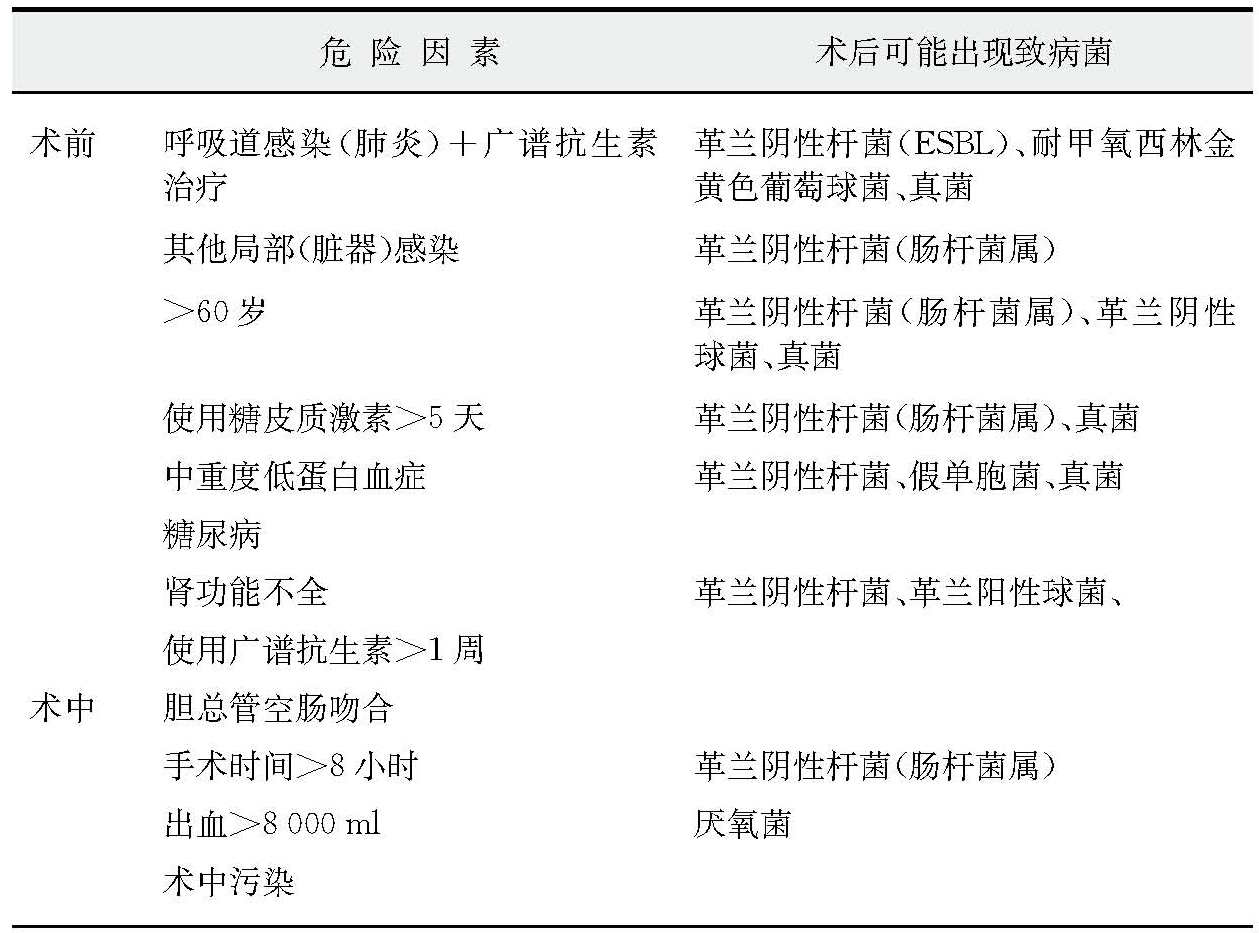
\includegraphics[width=\textwidth,height=\textheight,keepaspectratio]{./images/Image00112.jpg}
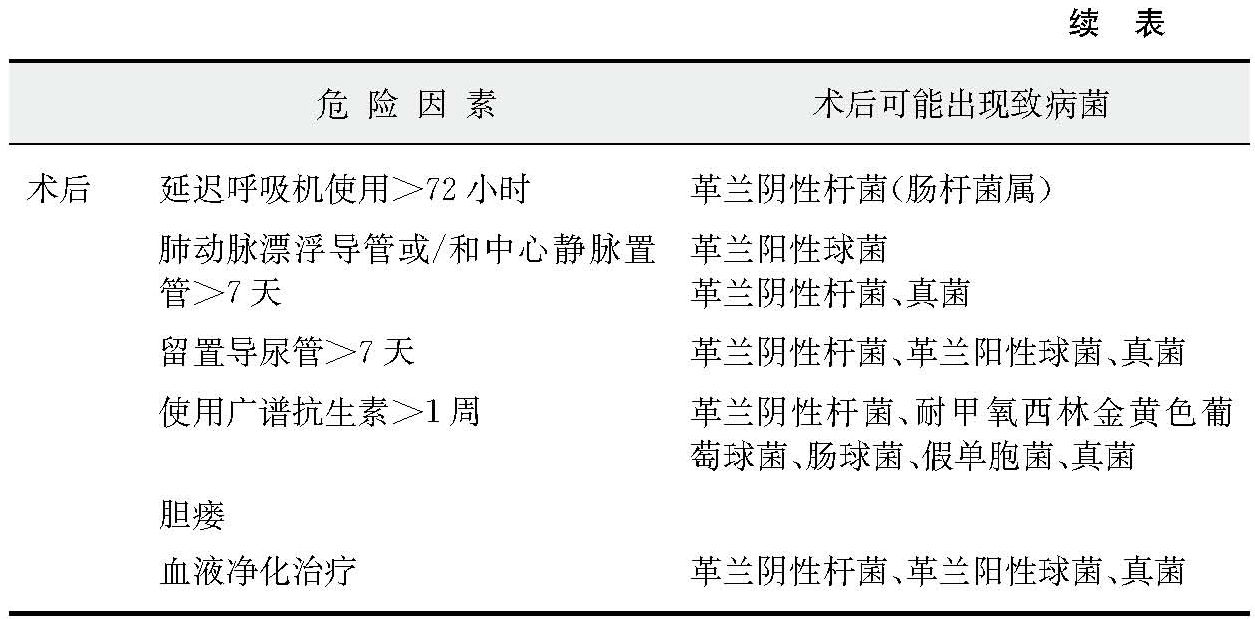
\includegraphics[width=\textwidth,height=\textheight,keepaspectratio]{./images/Image00113.jpg}
\end{table}

\subsubsection{肝移植围手术期的感染预防策略有哪些?}

根据术前、术中及术后危险因素(表\ref{tab14-3}),有无感染情况、出现感染的部位及感染程度,推荐下列抗感染药物预防感染方案。

如肝移植受体无表\ref{tab14-3}中列出的各项感染性并发症危险因素,手术当天术前使用一次抗感染药物,术中4~6小时加用一次(如术前使用头孢曲松,术中不必加用),预防性使用时间是术后3~5天,抗感染药物可选用氨苄青霉素、氧哌嗪青霉素、三代头孢(头孢曲松或头孢他啶)其中之一。

如肝移植受体出现表\ref{tab14-3}中列出的非感染性危险因素一项以上,手术当天术前使用一次抗感染药物,术中4~6小时加用一次,预防性使用时间是术后1周以内。抗感染药物可选用四代头孢(头孢吡肟)、加酶抑制剂药物(如梭苄青霉素+克拉维酸、氧哌嗪青霉素+他唑巴坦、头孢哌酮+舒巴坦中的一种)。此外,需加用抗真菌药物氟康唑。

如肝移植受体出现表\ref{tab14-3}中列出的危险因素中的感染性合并症,手术前延续抗感染药物治疗,术中4~6小时加用一次,术后根据感染有无进一步加重决定使用抗感染药物时间。此类患者宜在术前及时明确病原微生物及药物敏感实验结果,以利于准确选用抗感染药物。经验性抗感染药物可选用四代头孢(头孢吡肟)、加酶抑制剂抗感染药物(如梭苄青霉素+克拉维酸、氧哌嗪青霉素+他唑巴坦、头孢哌酮+舒巴坦中的一种)。此外,需加用抗真菌药物。

\subsubsection{肝移植术后如何应用经验性抗感染药物?}

经验应用抗感染药物宜选择对肝、肾损害较轻的药物,一般选青霉素类或头孢菌素类(慎用氨基糖苷类、大环内酯类)。

如肝移植受体无表\ref{tab14-3}所列出的各项危险因素,经验性预防感染药物可选用氨苄西林、哌拉西林、三代头抱(头孢曲松、头孢他啶等)。手术当天术前30分钟静脉滴注一次抗感染药物。如手术时间延长,术中每3~4小时加用一次。预防性使用时间是术后3~5天。

如肝移植受体出现表\ref{tab14-3}中所列出的危险因素一项以上,经验性预防感染药物可选用加酶抑制剂的抗生素(如氨苄西林+克拉维酸、呱拉西林+他唑巴坦、头孢哌酮+舒巴坦)、四代头孢(头孢吡肟马斯平),须加用抗真菌药物(氟康唑)。手术当天术前使用一次抗感染药物,术中每3~4小时加用一次,预防性使用时间是术后3~5天。

如肝移植受体出现表\ref{tab14-3}中所列出的危险因素中的感染性并发症,经验性预防感染药物可选用加酶抑制剂的抗感染药物(如替卡西林+克拉维酸、哌拉西林十他唑巴坦、头孢哌酮+舒巴坦)或四代头孢(头孢吡肟马斯平)。须加用抗真菌药物(氟康唑)。手术前应使用抗菌药物进行有效控制。手术开始前使用一次抗感染药物,术中每3~4小时加用一次,术后根据感染是否得到控制决定使用抗感染药物的时间。此类患者宜在术前及时明确病原微生物及药物敏感试验结果,以利于手术后准确选用抗感染药物。

\subsubsection{肝移植术后真菌感染的预防策略有哪些?}

肝移植术后真菌感染防治重点应放在提高早期诊断率,发现更有效、毒性更低的药物方面。肝移植术后应常规做痰培养,预防性应用抗真菌药物。有研究表明,氟康唑预防移植后念珠菌感染安全、有效。而曲霉、隐球菌防治措施尚未明确。预防性应用氟康唑(口服100mg/天×28天)可明显减少真菌集落形成和浅表真菌病,深部真菌感染亦有下降趋势。在此剂量下无肝毒性发生,未出现与环孢素相互作用引起的不良反应
\protect\hyperlink{text00020.htmlux5cux23ch62-19}{\textsuperscript{{[}62{]}}}
。

肝移植术后接受透析治疗的患者中,深部其他真菌和曲霉菌感染发生率(分别为36%和14%)明显高于无需透析患者(7%和2%)。预防性应用两性霉素脂质体后,接受透析治疗的肝移植患者深部真菌病发生率自36%(8/22例)降为0(0/11例),但病死率无降低。

对具有下列两种以上危险因素的肝移植患者,美国感染性疾病协会推荐预防应用抗真菌药(氟康唑或两性霉素B)------危险因素包括再移植、肌酐水平>2.0mg/dl、胆管空肠吻合术、应用>40U的血制品及移植后3天内真菌集落形成。

\subsection{肝脏移植术后重症医学科的监测与治疗}

\subsubsection{肝脏移植术后在重症医学科应重点监测哪些内容?}

肝移植手术后,患者转入重症医学科时,一般带有气管插管、漂浮导管及动脉测压导管。进入重症医学科病房后,负责接收患者的重症医学科医生和护士应当迅速连接好各种监测通道,并详细阅读麻醉单和手术记录,了解手术经过和麻醉方式,术中的详细情况(包括术中出血量、液体出入量、血流动力学参数、免疫抑制药的应用方案及术中发生的其他情况),并对患者的生命体征和各脏器功能做好评估、监测和管理。重症医学科内管理内容包括血流动力学、供肝功能、凝血功能、呼吸、神经、血液常规及生化、代谢、腹腔引流、免疫抑制剂用法、用量和浓度、感染情况等。

(1)血流动力学监测 术前及术后早期常规保留有创动脉压监测及Swan-Ganz肺动脉漂浮导管监测,目前新开展的监测手段还有脉波指示剂连续心排血量和微截流技术,通过监测平均动脉压、心排血量指数、心脏每搏射血指数、血管外肺水、肺血管阻力、外周血管阻力、左心室收缩功指数、氧输送等血流动力学及氧动力学等指标,对了解术前心功能储备、心脏前后负荷变化、判断术后是否存在心肌功能抑制及程度、全身氧输送及利用状况意义较大,也对术后多器官功能衰竭的发生率的评估具有特别重要的意义。

(2)供肝功能 术后有意义的供肝功能良好的指标有:患者神志清楚、各项肝功能指标正常、术前代谢性酸中毒(如果存在)纠正、凝血功能稳定和改善、体循环阻力稳定或逐步升高。目前肝移植常规均不留置T管,如因特殊原因有T管留置,则24~48小时内T管应引出金黄色胆汁。

(3)凝血功能监测 凝血因子的测定反映供肝的合成功能。术毕转入重症医学科应立即监测的凝血功能指标是凝血酶原时间、部分凝血活酶时间、血小板、全血细胞计数、D-D二聚体和纤维蛋白降解产物。

(4)出入量监测 有效循环血容量及每小时出入量、腹腔引流量监测,了解腹腔内液体丢失及有无持续性出血情况,术后第三间隙血容量丢失较常见,计量时应予以考虑。

(5)神经系统 包括知觉水平、脑神经反射及感觉功能,除此以外还应检测意识状态、定向力、瞳孔、生理反射和病理反射的变化。这些监测对于确定患者是否存在有爆发性肝衰竭极其重要。

(6)呼吸系统 包括动脉血气分析、经皮氧饱和度、呼吸频率等监测。动脉血气分析显得尤其重要。持续经皮氧饱和度监测对评估呼吸功能变化也很有价值,但是必须注意末梢循环差、严重黄疸或血管内染料对经皮氧饱和度测定的干扰。在呼吸机上可以检测到呼吸频率、气道压力的峰值和每分钟通气量。自主呼吸的出现是患者从麻醉状态开始复苏以及脑干功能良好的证据。气道压力增加提示肺顺应性降低,常见于术后肺间质水肿或胸腔积液。有时也可以由于腹腔张力过高影响膈肌活动所致。每分钟通气量增加提示通气死腔增加和二氧化碳产生增加,死腔增加可能的原因是肺梗死或低血容量;二氧化碳增加可以是复温的结果,而二氧化碳减少常发生于移植肝无功能、肝动脉血栓形成、超急性排斥引起的肝脏梗死等情况。

(7)肾功能监测 肾功能通过尿量、血浆尿素氮、肌酐、血肌酐清除率的监测来判定。术后肾功能影响因素要注意到3个方面:低有效循环血容量、CsA或FK506毒性作用以及术前存在的肾功能不全。

(8)腹部情况 各引流管内容物每24小时统计一次,若引流量偏多,每小时计量一次,并监测血红蛋白的变化情况。术后第一天常规行床边彩色多普勒超声检查,观察有无胸腔积液、腹腔积液、肝脏大小、胆管情况,行多普勒超声检查观察肝动脉和门静脉的血流情况,术后1周内可复查肝脏彩超,之后视具体情况选择性行彩色多普勒超声检查。

\begin{center}\rule{0.5\linewidth}{\linethickness}\end{center}

参考文献

\protect\hyperlink{text00020.htmlux5cux23ch1-19-back}{{[}1{]}} .Onaca
NN,Levy MF,Sanchez EQ,et al.A correlation between the
pretransplantation MELD score and mortality in the first two years after
liver transplantation.Liver Transpl,2003,9:117-123.

\protect\hyperlink{text00020.htmlux5cux23ch2-19-back}{{[}2{]}}
.谢琴芬,徐骁.第17届国际肝移植学会年会纪要.中华移植杂志(电子版).2011,5(3):247-249.

\protect\hyperlink{text00020.htmlux5cux23ch3-19-back}{{[}3{]}} .Douglas
DM,Abouass Ia,Habib A,et al.Persistent ascites and low serum sodium
identify patients with cirrhosis and low MELD scores who are at high
risk for early death.Hepatology,2004,40:802-810.

\protect\hyperlink{text00020.htmlux5cux23ch4-19-back}{{[}4{]}} .Biggins
SW,Rodriguez HJ,Bacchetti P,et al.Serum sodium predicts mortality in
patients listed for liver transplantation,Hepatology,2005,41:32-39.

{[}5{]}.Shear L,Kleinerman J,Gabuzda GJ.Renal failure in patients
with cirrhosis of the liver Clinical and pathological
characteristics.Am J Med,1965,39:184-198.

\protect\hyperlink{text00020.htmlux5cux23ch6-19-back}{{[}6{]}} .Cai
C-J,Chen H-A,Lu M-Q,et al.Model for en-stage liver disease-sodium
predicts prognosis in patients with chronic sever hepatitis B.Chi J
Med,2008,121(20):2065-2069.

\protect\hyperlink{text00020.htmlux5cux23ch7-19-back}{{[}7{]}} .Huo
T-I,Wang Y-W,Yang Y-Y,et al.Model for end-stage liver disease score
to serum sodium ratio index as a prognostic predictor and its
correlation with portal pressure in patients with liver cirrhosis.Liver
Int,2007,27:498-506.

\protect\hyperlink{text00020.htmlux5cux23ch8-19-back}{{[}8{]}} .Strong
RW,Lynch SV,Ong TH,et al.Successful liver transplantation from a
living donor to her son.N Engl J Med. 1990,322:1505-1507.

\protect\hyperlink{text00020.htmlux5cux23ch9-19-back}{{[}9{]}} .Yamaoka
Y,Washida M,Honda K,et al.Liver transplantation using a right lobe
graft from a living related donor.Transplantation,1994,57:1127-1130.

\protect\hyperlink{text00020.htmlux5cux23ch10-19-back}{{[}10{]}}
.Shiffman ML,Brown RS,Olthoff KM,et al.Living donor liver
transplantation:summary of a conference at The National Institutes of
Health.Liver Transpl,2002,8:174:188.

\protect\hyperlink{text00020.htmlux5cux23ch11-19-back}{{[}11{]}}
.Oldhafer KJ,Lang H,Schlitt HJ,et al.Long-term experience after ex
situ liver surgery.Surgery,2000,5,127(5):520-527.

\protect\hyperlink{text00020.htmlux5cux23ch12-19-back}{{[}12{]}} .Suh
KS,Lee HW,Shin WY,et al.Split Liver Transplantation.The Journal of
the Korean Society for Transplantation. 2007,21(1):135-139.

\protect\hyperlink{text00020.htmlux5cux23ch13-19-back}{{[}13{]}}
.Yersiz H,Cameron AM,Carmody I,et al.Split Liver
Transplantation.Transplant Proc. 2006,38(2):602-603.

\protect\hyperlink{text00020.htmlux5cux23ch14-19-back}{{[}14{]}}
.Deshpande RR,Bowles MJ,Vilca-Melendez H,et al.Results of Split
Liver Transplantation in Children.Ann surg.2002,8:248-253.

\protect\hyperlink{text00020.htmlux5cux23ch15-19-back}{{[}15{]}}
.CLTR.2009年中国肝移植年度科学报告[R].

\protect\hyperlink{text00020.htmlux5cux23ch16-19-back}{{[}16{]}}
.Casavilla A,Ramirez C,Shapiro R,et al.Experience with liver and
kidney allografts from non-heart-beating donors.Transplant
Proc,1995,27(5):2898.

\protect\hyperlink{text00020.htmlux5cux23ch17-19-back}{{[}17{]}}
.D'Alessandro AM,Hoffmann RM,Knechtle SJ,et al.Successful
extrarenal transplantation from non-heart-beating
donors.Transplantation,1995,59(7):977-982.

\protect\hyperlink{text00020.htmlux5cux23ch18-19-back}{{[}18{]}} .Foley
DP,Fernandez LA,Leverson G,et al.Donation after cardiac death:the
University of Wisconsin experience with liver transplantation.Ann
Surg,2005,242:724-731.

\protect\hyperlink{text00020.htmlux5cux23ch19-19-back}{{[}19{]}}
.Nguyen JH,Bonatti H,Dickson RC,et al.Long-term outcomes of
donation after cardica death liver allografts from a single center.Clin
Transplant,2009,23:168-173.

\protect\hyperlink{text00020.htmlux5cux23ch20-19-back}{{[}20{]}} .Detry
O,Seydel B,Delbouille MH,et al.Liver transplant donation after
cardiac death:experience at the University of Liege.Transplant
Proc,2009,41:582-584.

\protect\hyperlink{text00020.htmlux5cux23ch21-19-back}{{[}21{]}}
.管向东,黄洁夫,陈秉学等.原位肝移植术后早期管理体会.新医学,1997,10:214-216.

\protect\hyperlink{text00020.htmlux5cux23ch22-19-back}{{[}22{]}}
.Uemura T,Randall HB,Sanchez EQ.Liver retransplantation for primary
nonfunction:analysis of a 20-year single-center experience.Liver
Transpl,2007,13(2):227-233.

\protect\hyperlink{text00020.htmlux5cux23ch23-19-back}{{[}23{]}} .Rull
R,Vidal O,Momblan D,et al.Evaluation of potential liver
donors:limits imposed by donor variables in liver
transplantation.Liver Transpl,2003,9:389-393.

\protect\hyperlink{text00020.htmlux5cux23ch24-19-back}{{[}24{]}}
.Tassani P,Schad H,Winkler C,et al.Capillary leak syndrome after
cardiopulmonary bypass in elective,uncomplicated coronary artery bypass
grafting operations:does it exist?J Thorac Cardiovasc
Surg,2002,123(4):735-741.

\protect\hyperlink{text00020.htmlux5cux23ch25-19-back}{{[}25{]}}
.Manthous CA,Amoatent Y,et al.Negative fluid balance as predictor of
mortality.Chest,2000,120:1424-1425.

{[}26{]}.Therapondos G,Flapan AD,Plevris JN and Hayes PC.Cardiac
morbidity and mortality related to orthotopic liver
transplantation.Liver Transplantation,2004;10(12):1441-1453.

{[}27{]}.McGilvrary ID,Greig PD,Critical care of the liver
transplantation patient:an update.Current Opinion in Critical
Care,2002,8:178-182.

\protect\hyperlink{text00020.htmlux5cux23ch28-19-back}{{[}28{]}}
.Wiklund RA.Preoperative preparation if patients with advanced liver
disease.Crit Care Med,2004;32(4 suppl.):S106-115.

\protect\hyperlink{text00020.htmlux5cux23ch29-19-back}{{[}29{]}}
.Cannesson M,Musard H,Desebbe O,et al.The ability of stroke volume
variations obtained with Vigileo/Flo Trac system to monitor fluid
responsiveness in mechanically ventilated patients.Anesth Analg.
2009,108(2):13-517.

\protect\hyperlink{text00020.htmlux5cux23ch30-19-back}{{[}30{]}}
.姚尚龙,尚游.每搏输出量变异度功能性血流动力学监测的重要指标.中华生物医学工程杂志,2008,14(4):241-243.

\protect\hyperlink{text00020.htmlux5cux23ch31-19-back}{{[}31{]}}
.王合梅,贾慧群,雍芳芳,等.每搏量变异度与患者血容量变化的相关性.中华麻醉学杂志,2010,30(7):914-916.

\protect\hyperlink{text00020.htmlux5cux23ch32-19-back}{{[}32{]}}
.Zimmermann M,Feibicke T,Keyl C,et al.Accuracy of stroke volume
variation compared with pleth variability index to predict fluid
responsiveness in mechanically ventilated patients undergoing major
surgery.Eur J Anaesthesiol,2010,27(6):555-561.

\protect\hyperlink{text00020.htmlux5cux23ch33-19-back}{{[}33{]}}
.管向东,陈规划,黄文起,等.原位肝移植术后早期超正常化氧输送对患者预后影响的研究.中国实用外科杂志,2001,11:321-322.

\protect\hyperlink{text00020.htmlux5cux23ch34-19-back}{{[}34{]}}
.吴健锋,管向东,陈娟,等.24h乳酸清除率预测肝移植早期发生并发症临床价值研究.中国实用外科杂志,2011,32(4):325-327.

\protect\hyperlink{text00020.htmlux5cux23ch35-19-back}{{[}35{]}}
.徐向东,吴健锋,管向东,等.早期乳酸清除率评估外科严重脓毒症预后的临床价值研究.中国实用外科杂志,2007,27(12):969-970.

\protect\hyperlink{text00020.htmlux5cux23ch36-19-back}{{[}36{]}}
.Tomasdottir H,Bengtson JP,Bengtsson A.Neutrophil and macrophage
actviation and anaphylatoxin formation in orthotopic liver
transplantation without the use of veno-venous bypass.Acta
Anaeasthesiol.Scand,1996,40:250-255.

\protect\hyperlink{text00020.htmlux5cux23ch37-19-back}{{[}37{]}} .Segal
H,Sheikh S,Kallis P,et al.Complement activation during major
surgery:the effect of extracorporeal circuits and high dose
aprotinin.J Cardiothorac Vasc Anesth,1998,12:542-547.

\protect\hyperlink{text00020.htmlux5cux23ch38-19-back}{{[}38{]}}
.Arvidsson D,Almquist P,Haglund U.Effects of positive end expiratory
pressure on splanchnic circulation and function in experimental
perionitis.Arch Surg,1991,126:631-636.

\protect\hyperlink{text00020.htmlux5cux23ch39-19-back}{{[}39{]}}
.Clause GK,Peter K,Bruno S,et al.Effects of positive end-expiratory
pressure on hemodynamics and indocyanine green kinetics inpatients after
orthotopic liver transplantation.Crit Care Med,2000,28:1760-1765.

\protect\hyperlink{text00020.htmlux5cux23ch40-19-back}{{[}40{]}} .Ghaus
N,Bohlega S,Rezeig M.Neurological complications in liver
transplantation.J Neurol,2001,248:1042-1048.

{[}41{]}.Araz C,Pirat A,Torgay A,et al.Early postoperative
complications of pediatric liver transplantation:experience at one
center.Transplant Proc,2004,36:214-217.

\protect\hyperlink{text00020.htmlux5cux23ch42-19-back}{{[}42{]}}
.蔡常洁,陆敏强,安玉玲,等.肝移植术后并发桥脑中央髓鞘溶解症的诊断和治疗.南方医科大学学报,2007,27(6):849-851.

\protect\hyperlink{text00020.htmlux5cux23ch43-19-back}{{[}43{]}}
.Mueller AR,Platz KP,Bechstein WO,et al.Neurotoxicity after
orthotropic liver
transplantation.Transplantation,1994,58(2):155-170.

\protect\hyperlink{text00020.htmlux5cux23ch44-19-back}{{[}44{]}} .Jain
A,Brody D,Hamad D,et al.Conversion to neoral for neurotoxicity after
primary adult liver transplantation under
tacrolimus.Transplantation,2000,69(1):172-176.

\protect\hyperlink{text00020.htmlux5cux23ch45-19-back}{{[}45{]}}
.蔡常洁,陆敏强,李敏如,等.重型肝炎患者肝移植术后细菌感染的防治.中华普通外科杂志,2006,21(11):804-806.

\protect\hyperlink{text00020.htmlux5cux23ch46-19-back}{{[}46{]}}
.蔡常洁.外科危重患者代谢改变及其对临床营养的指导.中国实用外科杂志,2012,32(2):125-127.

\protect\hyperlink{text00020.htmlux5cux23ch47-19-back}{{[}47{]}}
.蔡常洁,陈规划,管向东,等.肝移植术后细菌感染的流行病学分析.中国实用外科杂志,2003,23:163-164.

\protect\hyperlink{text00020.htmlux5cux23ch48-19-back}{{[}48{]}} .Rubin
RH.The direct and indirect effects of infection in liver
transplantation:pathogenesis,impact,and clinical management.Curr
Clin Top Infect Dis,2002,22:125-154.

\protect\hyperlink{text00020.htmlux5cux23ch49-19-back}{{[}49{]}}
.Tachopoulou OA,Vogt DP,Henderson JM,et al.Hepatic abscess after
liver transplantation:1990-2000.Transplantation,2003,75:79-83.

\protect\hyperlink{text00020.htmlux5cux23ch50-19-back}{{[}50{]}}
.Koivusalo A,Isoniemi H,Salmela K,et al.Biliary complications in
100 adult liver transplantations:a retrospective clinical
study.Transpl Int,1994,7(Suppl1):S119-S120.

\protect\hyperlink{text00020.htmlux5cux23ch51-19-back}{{[}51{]}}
.Alessiani M,Kusne S,Martin FM,et al.Infection with FK506
immunosuppression:preliminary results with primary therapy.Transplant
Proc,1990,22:44-46.

\protect\hyperlink{text00020.htmlux5cux23ch52-19-back}{{[}52{]}}
.Fishman JA,Rubin RH.Infection in organ-transplant recipients.N Engl
J Med,1998,338:1741-1751.

\protect\hyperlink{text00020.htmlux5cux23ch53-19-back}{{[}53{]}} .Blair
JE,Kusne S.Bacterial,mycobacterial,and protozoal infections after
liver transplantation partⅠ.Liver Transplant,2005,11:1452-1459.

\protect\hyperlink{text00020.htmlux5cux23ch54-19-back}{{[}54{]}} .Rubin
RH,Young LS.Clinical approach to infection in the compromised
host.New York:Kluwer Academic/Plenum,2002:573-679.

\protect\hyperlink{text00020.htmlux5cux23ch55-19-back}{{[}55{]}} .Liu
X,Ling Z,Li L,et al.Invasive fungal infections in liver
transplantation.Int J Infect Dis,2011,15:e298-304.

\protect\hyperlink{text00020.htmlux5cux23ch56-19-back}{{[}56{]}} .Hoppe
CA,Marroni R,Bressane L,et al.Risk factors associated with
cytomegalovirus infection in orthotopic liver transplant
patients.Transplant Proc,2006,38:1922-1923.

\protect\hyperlink{text00020.htmlux5cux23ch57-19-back}{{[}57{]}}
.蔡常洁,陆敏强,杨扬,等.肝移植术后巨细胞病毒性肺炎的临床特点和治疗方法.中华器官移植杂志,2006,27(6):361-363.

\protect\hyperlink{text00020.htmlux5cux23ch58-19-back}{{[}58{]}}
.Sanchez A,Larsen R.Fungal infections in solid organ
transplantation.Curr Opin Organ Transplant,2007,12:579-584.

\protect\hyperlink{text00020.htmlux5cux23ch59-19-back}{{[}59{]}} .Blair
JE.Coccidioidomycosis in liver transplant transplantation.Liver
Transpl,2006,12:31-39.

\protect\hyperlink{text00020.htmlux5cux23ch60-19-back}{{[}60{]}}
.Sachdev MS,Blair JE,Mulligan DC,Kusne S.Coccidioidomycosis masked
by symptoms of end-stage lever disease in transplant
candidates.Transplant Inf Dis,2007,9:153-155.

\protect\hyperlink{text00020.htmlux5cux23ch61-19-back}{{[}61{]}} .Oh
YS,Lisker-Melman M,Korenblat KM,et al.Disseminated histoplasmosis in
a liver transplant recipient.Liver Transplant,2006,12:677-681.

\protect\hyperlink{text00020.htmlux5cux23ch62-19-back}{{[}62{]}}
.蔡常洁,李敏如,陆敏强,等.肝移植术后真菌感染的防治新策略.中国实用外科杂志,2007,27(1):78-80.

\protect\hypertarget{text00021.html}{}{}

